\section{V1 Receptive Fields Construction}
\label{sec:aMechanisticModel}

\begin{rem}
  The models of visual receptive fields we have been discussing are purely descriptive, but they provide an important framework for studying how the circuits of the retina, LGN, and primary visual cortex generate neural responses.
\end{rem}

\begin{defn}
  \label{defn:Hubel-WieselSimpleCellModel}
  The \emph{Hubel-Wiesel Model} propose the oriented receptive fields of cortical neurons could be generated by summing the input from appropriately selected LGN neurons.
\end{defn}

\begin{exm}[The Hubel-Wiesel model of a simple cell]
  \label{exm:simpleCellModel}
  The Hubel-Wiesel model of orientation selectivity is shown below.
  \begin{center}
    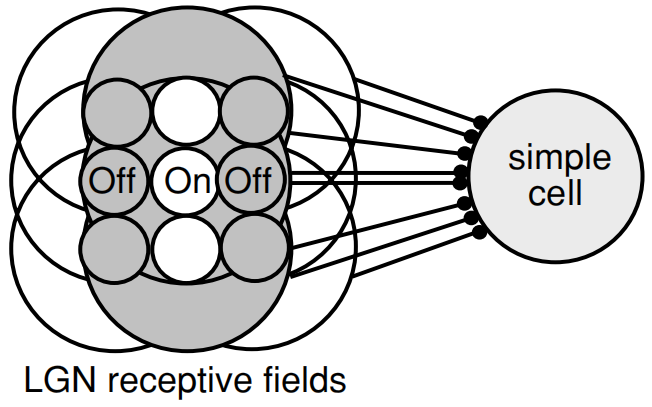
\includegraphics[scale=0.2]{./png/simpleCellModel}
  \end{center}
  The spatial arrangement of the receptive fields of nine LGN neurons are shown, with a column of three ON-center fields flanked on either side by columns of three OFF-center fields. White areas denote ON fields and gray areas, OFF fields. In the model, the converging LGN inputs are summed by the simple cell. \emph{This arrangement produces a receptive field oriented in the vertical direction.} Note that, two center types are represented as
  \begin{enumerate}[(i)]
  \item ON-center field: a concentric circle with an white inner circle and an gray outer circle;
  \item OFF-center field: a concentric circle with an gray inner circle and an white outer circle.
  \end{enumerate}
\end{exm}

\begin{rem}
  This model accounts for the selectivity of a simple cell purely on the basis of feedforward input from the LGN.
\end{rem}

\begin{rem}
  In a previous section, we showed how the properties of complex cell responses could be accounted for by using a squaring static nonlinearity. While this provides a good description of complex cells, there is little indication that complex cells actually square their inputs. Models of complex cells can be constructed without introducing a squaring nonlinearity.
\end{rem}

\begin{exm}[The Hubel-Wiesel model of a complex cell]
  \label{exm:complexCellModel}
   Inputs from a number of simple cells with similar orientation and
spatial frequency preferences ($\theta$ and $k$), but different spatial phase preferences ($\phi_1$, $\phi_2$, $\phi_3$, and $\phi_4$), converge on a complex cell and are summed. \emph{This produces a complex cell output that is selective for orientation and spatial frequency, but not for spatial phase (phase-invariant response).}
  \begin{center}
    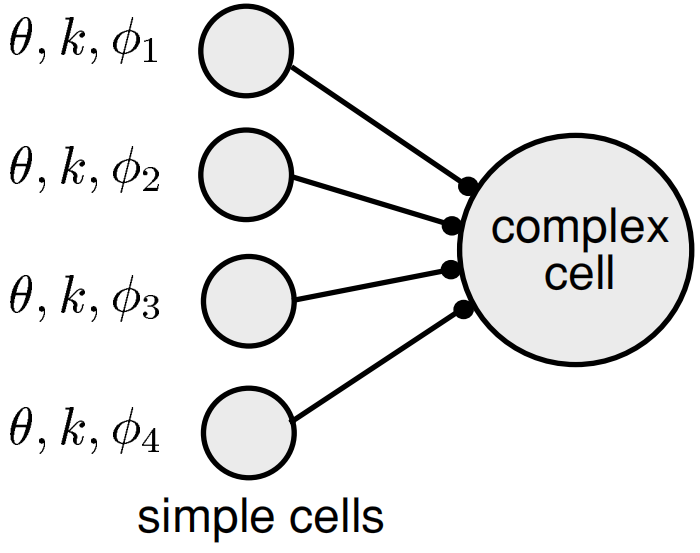
\includegraphics[scale=0.18]{./png/complexCellModel}
  \end{center}
  The figure shows four simple cells converging on a complex cell, but additional simple cells can be included to give a more complete coverage of spatial phase.
\end{exm}

%\begin{rem}
  %In this model of Example \ref{exm:complexCellModel}, the complex cell inherits its orientation and spatial frequency preference from the simple cells that drive it, but spatial phase selectivity is reduced because the outputs of simple cells with a variety of spatial phase selectivities are summed.
%\end{rem}

\begin{rem}
   While the model generates complex cell responses, there are indications that complex cells in primary visual cortex are not driven exclusively by simple cell input. An alternative model is considered in chapter 7.
\end{rem}

%%% Local Variables:
%%% mode: latex
%%% TeX-master: "../notesOnFluidMechanics"
%%% End:
